\documentclass[a4]{article}

\usepackage[left=3cm,right=3cm,top=2cm,bottom=2cm]{geometry} 

\usepackage[utf8]{inputenc}   % otra alternativa para los caracteres acentuados y la "ñ"
\usepackage[           spanish % para poder usar el español
                      ,es-tabla % para los captions de las tablas
                       ]{babel}   
\decimalpoint %para usar el punto decimal en vez de coma para los números con decimales

\usepackage[T1]{fontenc}
\usepackage{lmodern}

\usepackage{parskip}
\usepackage{xcolor}

\usepackage{caption}

\usepackage{enumerate} % paquete para poder personalizar fácilmente la apariencia de las listas enumerativas

\usepackage{graphicx} % figuras
\usepackage{subfigure} % subfiguras

\usepackage{amsfonts}
\usepackage{amsmath}

\definecolor{gris}{RGB}{220,220,220}
	
\usepackage{float} % para controlar la situación de los entornos flotantes

\restylefloat{figure}
\restylefloat{table} 

\newcommand{\HRule}{\rule{\linewidth}{0.5mm}}

\author{David Cabezas Berrido}
\date{\vspace{-5mm}}

\title{\huge Práctica 1 \HRule\vspace{-4mm}}

\begin{document}
\maketitle
\tableofcontents

\section{Ejercicio sobre la búsqueda iterativa de óptimos: \\ Gradiente descendiente}

\subsection{Minimizar la función $E(u,v)$}

La función a minimizar es $E(u,v)=(ue^v-2ve^{-u})^2$, le aplicamos el algoritmo del gradiente 
descendente partiendo del punto $w=(1,1)$ con tasa de aprendizaje $\eta=0.1$.
La función es no negativa y sabemos que si encontramos un cero será un mínimo absoluto,
aceptamos un margen de error $\varepsilon=10^{-14}$ y nos interesa el punto en el que se alcanza
y las iteraciones necesarias para alcanzarlo. También he fijado un máximo de 100 iteraciones,
ya que no tengo asegurado encontrar un 0 y hay que añadir esa condición para asegurarnos
de que va a parar en algún momento.

He usado la librería \texttt{sympy} para el cálculo de las derivadas parciales en el programa.
También las he calculado analíticamente y el gradiente queda de este modo:

\begin{equation*}
\nabla E(u,v)=
\begin{pmatrix}
\frac{\partial E}{\partial u}(u,v) \vspace{2mm}\\
\frac{\partial E}{\partial v}(u,v)
\end{pmatrix}=
\begin{pmatrix}
    2(ue^v-2ve^{-u})(e^v+2ve^{-u}) \vspace{2mm}\\
    2(ue^v-2ve^{-u})(ue^v-2e^{-u})
    \end{pmatrix}
\end{equation*}

He ejecutado el algoritmo y, en sólo 10 iteraciones, he encontrado un valor por debajo de $\varepsilon$,
en el punto $w=(0.0447362903977822,0.0239587140991418)$.

\subsection{Estudio de la dependencia del \textbf{learning rate} ($\eta$)}

He utilizado el algoritmo del gradiente descendente para buscar un mínimo local de la función \\
$f(x,y)=(x-2)^2+2(y+2)^2+2\sin(2\pi x)\sin(2\pi y)$ partiendo desde el punto $(1,-1)$. Esta vez
realiza un número de iteraciones fijo (50 iteraciones), ya que desconozco los valores que puede
tomar la función y no puedo incorporar un criterio de parada como el de antes. Sí que podría incluir
como criterio la norma del gradiente, ya que ésta es casi 0 cuando estamos muy cerca del mínimo local.

El objetivo ésta vez es estudiar cómo afecta a la eficacia del algoritmo el valor escogido para la
tasa de aprendizaje $\eta$, para ello he ejecutado el algoritmo con dos valores diferentes de $\eta$
(0.01 y 0.1) y he medido el valor de la función en cada iteración, para estudiar la velocidad a la que
decrece o si se salta el mínimo y vuelve a crecer. En las siguientes gráficas se muestra cómo evoluciona
el valor de la función en cada iteración.

\begin{figure}[H]
    \centering    
    \subfigure[$\eta=0.01$]{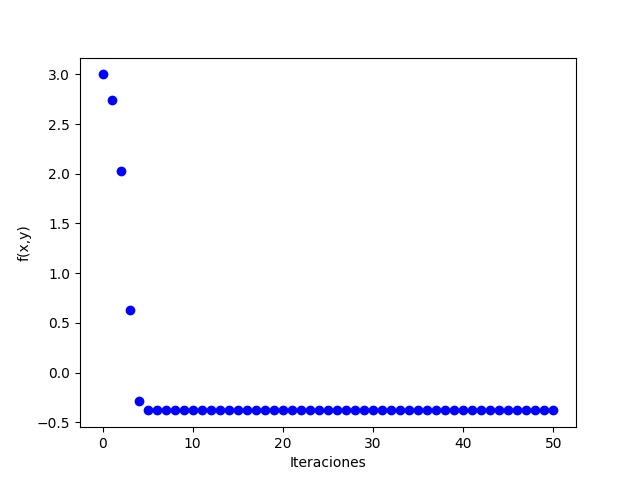
\includegraphics[width=77mm]{imgs/gd_0,01.png}}
    \subfigure[$\eta=0.1$]{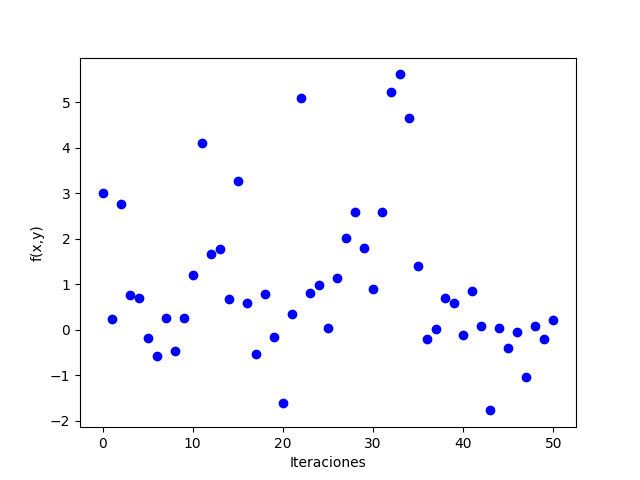
\includegraphics[width=77mm]{imgs/gd_0,1.png}}
    \caption{Comparación de la eficacia del algoritmo para dos valores de $\eta$.}
    \label{fig:comp-eta}
\end{figure}

Lo deseable es que la función decrezca lo más rápido posible. En el primer caso ($\eta=0.01$) se llega a un mínimo local
bastante rápido (se queda muy cerca en la quinta iteración) en el que la función toma el valor $-0.38124949743810027$,
en la segunda gráfica se aprecian valores de la función cercanos a -2, luego está claro que ese mínimo no es absoluto.

En cambio, la tasa de aprendizaje $\eta=0.1$ es demasiado alta y esto provoca que se salte el punto donde se alcanza el
mínimo local y el algoritmo no converja en el segundo caso. Es importante que la tasa de aprendizaje no sea demasiado alta
para evitar esto.

\subsection{Estudio de la dependencia del punto inicial escogido}

He ejecutado el algoritmo del gradiente descendiente para localizar mínimos locales en la función $f(x,y)$ partiendo
de distintas condiciones iniciales. Como no se especifica, he realizado 50 iteraciones y he fijado el valor $\eta=0.01$
como learning rate. He obtenido los siguientes resultados:

\begin{table}[H]
    \begin{tabular}{|c|l|c|}
    \hline
                 & $(x,y)$ donde se alcanza el mínimo & $f(x,y)$                                        \\ \hline
    $(2.1,-2.1)$ & -1.8200785415471563                & $( 2.2438049693647883 ,  -2.2379258214861775 )$ \\ \hline
    $(3,-3)$     & -0.38124949743810005               & $( 2.730935648248105 ,  -2.7132791261667033 )$  \\ \hline
    $(1.5,1.5)$  & 18.042078009957635                 & $( 1.7779244744891156 ,  1.032056872669696 )$   \\ \hline
    $(1,-1)$     & -0.38124949743810027               & $( 1.269064351751895 ,  -1.2867208738332965 )$  \\ \hline
    \end{tabular}
\end{table}

El algoritmo ha encontrado mínimos locales con valores muy diversos, lo que deja claro la dependencia del punto inicial.
Partiendo del punto $(1.5,1.5)$ he obtenido a una solución pésima, ya que ha quedado atrapado en un mínimo local con un
valor muy elevado. En cambio, partiendo del $(2.1,-2.1)$ he obtenido un
valor bastante cercano al mínimo absoluto, valor que no he obtenido con ninguna de las otras dos condiciones iniciales.
En este problema sé qué soluciones son buenas y cuales son malas porque he podido visualizar la función, pero en el caso
bastante común de que el espacio de funciones candidatas tenga dimensión mayor (haya que ajustar más de dos parámetros)
habría que minimizar una función de error que no se puede visualizar. Por tanto, el mínimo absoluto de una función de
varias variables es muy difícil de encontrar con certeza, a no ser que la función sea convexa. 

\section{Ejercicio sobre regresión lineal}
\end{document} 